\documentclass[12pt]{article}
\usepackage{amsmath}
\usepackage{authblk}
\usepackage[utf8]{inputenc}
\usepackage{subcaption}
\usepackage{natbib}
\usepackage{graphicx}
\usepackage{breqn}
\usepackage{float}
\restylefloat{table}
\usepackage{array}
\usepackage[hidelinks]{hyperref}
\usepackage[table]{xcolor}% http://ctan.org/pkg/xcolor
\setlength{\parindent}{0pt}


\usepackage[a4paper,width=165mm,top=25mm,bottom=25mm]{geometry}
\graphicspath{ {./Pictures/} }
\title{\Huge Final User Test}
\author{Axel Trolme}

\begin{document}
\maketitle
\vfill

\includegraphics[width=\linewidth]{Pictures/logo_heartbyte_transparent_v_1_1.png}

\vfill
\begin{center}
        \textbf{\large Current Version 3.0 [2020-12-06]}
\end{center}
\clearpage

\section{Change Log}
	
\begin{table}[H]

\begin{center}
\begin{tabular}{ | m{2cm} |m{2cm} |m{5cm}|m{4cm}|m{3cm}| } 
\hline
{Version Number} & {Published Date} & {Description of Revision}& {Author}& {Approved By} \\ 
\hline
1.0 & 2020-12-02 & First version of the final user test plan & Axel Trolme & Emma Johansson \\
\hline
2.0 & 2020-12-04 & Added process description for how lostness is to be validated & Axel Trolme & Emma Johansson \\
\hline
3.0 & 2020-12-06 & Final result and calculations added & Axel Trolme & Emma Johansson \\
\hline
\end{tabular}
\end{center}
\caption{\label{tab:changeLog}Document change log}
\end{table}
\clearpage
\tableofcontents
\clearpage

% Introduction
    \section{Final user test background}
    The final user test is a test to be pursued with the intended end users of the system or a group of people with applicable information \& knowledge in the subject. Applicable information \& knowledge means that the person taking the test has to know the purpose of the system, as well as basic knowledge for navigating in a web application. \\ 
    
    The main purpose for the final user test is to validate if the developed product / system satisfies the non-functional requirements stated by the customer, in this case Region Östergötland. These non-functional requirements are to be found in the table below. The test is to focus on the usability aspects of the system as well as lostness, and is therefore mostly designed as a SUS-test while having processes for measuring lostness as well. Description for how the test is created and pursued is to be found under section \ref{sec: Method}. 
    \begin{table}[H]

    \begin{center}
    \begin{tabular}{ | m{2cm} |m{10cm} |m{2cm}| }  
    \hline
    \textbf{ID:} & \textbf{Statement} & \textbf{Priority} \\
    \hline
    NFR008 & 
    90\% of the system users shall perceive the system as easy to use and flexible. & 
    Low \\ 
    \hline
    NFR012 & 
    The Google Material Design system themed with Region Östergötland’s color palette shall be used. & 
    Medium \\ 
    \hline
    NFR016 & 
    The system shall be easy to navigate (have a low Lostness-score, i.e. $< 0.4$) &
    Low \\ 
    \hline
    NFR017 & 
    The system shall provide good user experience (have high SUS-score, i.e. $> 68$) & 
    Low \\ 
    \hline
    NFR018 & 
    The system shall be accessible for people with disabilities and follow WCAG guidelines. &
    Low \\ 
    \hline
    \end{tabular}
    \end{center}
    \caption{\label{tab:NFRs}Non-functional requirements to be tested with the user test}
    \end{table}
    \section{Method}
    \label{sec: Method}
    The test is divided into three different sections:
    
    \begin{enumerate}
        \item Inform the respondent thoroughly about the backstory to the project - why the system is created and its intended use. 
        \item Let the respondent perform the following tasks within the application in order to familiarise with the application and test its usability as well as lostness:
        \begin{enumerate}
            \item Find the latest notification from Gunilla Andersson and interact with her health data
            \item Find where to manually add a new weight measurement for Gunilla
            \item Find Gunilla's credentials (telephone number, address etcetera)
            \item Filter the patient list to only show diabetes patients.
            \item Filter the patient list to only show patient of high priority / urgent need of help.
            \item Find when Gunilla has her next appointment with a doctor.
            \item Find all the notifications for high priority patients.
        \end{enumerate}
        Every task is to be started from the patient view in this way, a value for lostness can be obtained by counting the number of views visited in order to fulfill the task. More information on this is to be found under section \ref{sec: lostness}.
        \item Let the respondent answer the SUS questions stated in section \ref{ref: Questions}.
    \end{enumerate}
    SUS is an abbreviation for System Usability Scale, and gives a good idea of how usable the system is experienced by its intended users. The test is built up by a questionnaire containing ten questions regarding the system. Five of these questions are to be positive statements and the other five are to be negative. The questions used in this very test are to be found under section \ref{ref: Questions}. This kind of test is often good to use when questions regarding usability for a web application is to be answered. \\
    
    The perks of using the SUS-test standard is mostly its easy set up and good coverage of the usability aspect. The ten questions listed under section \ref{ref: Questions} are to be answered on a scale from one to five, where one is to be interpreted as "I strongly disagree" and five as "I strongly agree". How the result from the test is calculated is to be found under section \ref{ref: Calculations}. 
    
    \subsection{Lostness}
    \label{sec: lostness}
    Lostness is a measurement to find out if the web application is built up in a logical way or if the layout has any major limitations. Through counting the number of views visited by the user in order to fulfil a certain task and compare this number with the optimal number of views visited, a value of lostness can be obtained. Through thousand of tests pursued in this way, it has been proven that a value below 0,4 is to be seen as good according to \href{https://uxdesign.cc/ux-metric-lostness-524998ccb215}{\underline{uxdesign.cc}}. The metric is calculated with the following formula: \\
    \begin{center}
          $N = Number \; of \; different\; visited \; views$ \\ $\; S = Total \; number \; of \; views\;visited$ \\ $ R = Minimum \; number \; of \; views\;visited \;,$
    \end{center}
  
    \begin{equation}
        Lostness = \sqrt{(\frac{N}{S}-1)^2 + \frac({R}{N}-1)^2}
    \end{equation}
    
    \subsection{Questions}
    \label{ref: Questions}
    
    According to \href{https://www.usability.gov/how-to-and-tools/methods/system-usability-scale.html}{\underline{Usability.gov}}, the following ten questions are to be answered when performing the SUS-test by each respondent: 
    
    \begin{enumerate}
        \item I think that I would like to use this system frequently.
        \item I found the system unnecessarily complex.
        \item I thought the system was easy to use.
        \item I think that I would need the support of a technical person to be able to use this system.
        \item I found the various functions in this system were well integrated.
        \item I thought there was too much inconsistency in this system.
        \item I would imagine that most people would learn to use this system very quickly.
        \item I found the system very cumbersome to use.
        \item I felt very confident using the system.
        \item I needed to learn a lot of things before I could get going with this system.
    \end{enumerate}
    \subsection{Calculation of the SUS - result}
    In order to get a result from the test, the answers from the respondents are validated. See the equations below for how this is done. The positive statements are numbered with uneven numbers $(1, 3, 5, 7, 9)$ and the negative statements are numbered with even numbers $(2, 4, 6, 8, 10)$. The resulting calculation is denoted $X_{i,Positive}$ for $ i = \{1,3,5,7,9\}$ and $X_{i,Negative}$ for $ i = \{2,4,6,8,10\}$. $Y_i = $ The answered number on question $ i = \{1,..,10\}$.

     \begin{equation}
        X_{i,Positive} = Y_i - 1 \;, \;for \;i = \{1,3,5,7,9\} \; \;else\;  X_{i,Positive} = 0
     \end{equation}
    
     \begin{equation}
         X_{i,Negative} = 5 - Y_i \;,\; i = \{2,4,6,8,10\}  \;else\;  X_{i,Negative} = 0
     \end{equation}
     
\begin{center}
    The resulting number for each respondent is then calculated as: 
\end{center}     
     
     \begin{equation}
         {Final\;result}_{\;one\;respondent} =  (\sum_{i=1}^{10} X_{i,Negative} + X_{i,Positive} ) \times 2,5 
     \end{equation}
   
    The result will end up between zero and 100. According to usability.gov (https://www.usability.gov/how-to-and-tools/methods/system-usability-scale.html), a result above 68 is seen as above average and above 86 is seen as good. These limits and numbers are statistically based on thousands of tests pursued in the past in various projects. The same source gives an idea about how many respondents that has to take the test in order to deliver a viable end result, with numbers varying from 2 to 50. In this test, ten respondents will participate The summarised result from all the respondents is to be found under section \ref{sec: Conclusion}.
   
    \label{ref: Calculations}
    \section{Conclusion \& result}
    \label{sec: Conclusion}
    From the answers from ten different respondents that is to be found under section \ref{sec: Answers}, the results to be found in the table below has been calculated. As a conclusion, we can see that most of the non-functional requirements to be found in table \ref{tab:NFRs} has been tested and taken into account - with a high success rate. The majority of the respondents (90\%) have received a SUS-score greater than 68 why NFR017 is to be seen as fulfilled. 100\% of the respondents answers that they find the system to be easy to use and flexible, why NFR008 is seen as fulfilled as well. All the respondents received a lostness-score lower than 0,4 why NFR016 is seen as fulfilled. NFR012 is also fulfilled and NFR018 has not been given any attention due to lack of time. 
    \begin{table}[H]

    \begin{center}
    \begin{tabular}{ | m{12cm} |m{3cm}|}  
    \hline
    \textbf{Measurement} & \textbf{Value} \\
    \hline
    Average SUS-score & 79,5 \\
    \hline
    Lowest SUS-score & 67,5\\
    \hline
	Highest SUS-score & 95 \\
    \hline				
    Median SUS-score & 81,25 \\
    \hline				
    Share of respondents with SUS-score \geq 68 & 90\% \\
    \hline
     & \\
    \hline
    Average lostness-score & 0,1\\
    \hline			
    Highest lostness-score & 0,3\\
    \hline				
    Lowest lostness-score & 0,1\\
    \hline				
    Median lostness-score & 0,1\\
    \hline
    & \\
    \hline
    Share of respondents finding the system easy to use & 100\%\\
    \hline				
    \end{tabular}
    \end{center}
    \caption{\label{tab:Reults}Calculated results from the final user-test}
    \end{table}
    
    
    
    
    
    \section{Appendix}
    Supporting data and relevant information connected to the execution of the final user test is to be found below. 
    \subsection{Answers from the respondents}
    \label{sec: Answers}
    \begin{figure}[H]
        \centering
        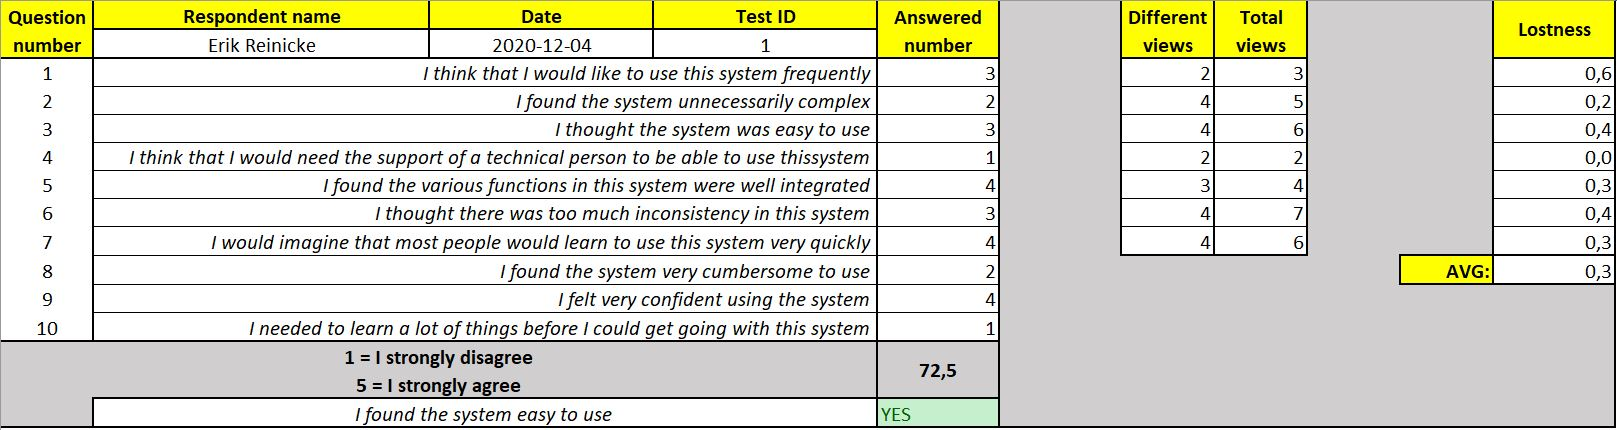
\includegraphics[width=\linewidth]{Pictures/Usertest_1.JPG}
        \caption{Answers from respondent 1}
        \label{fig:Usertest_1}
    \end{figure}
    \begin{figure}[H]
        \centering
        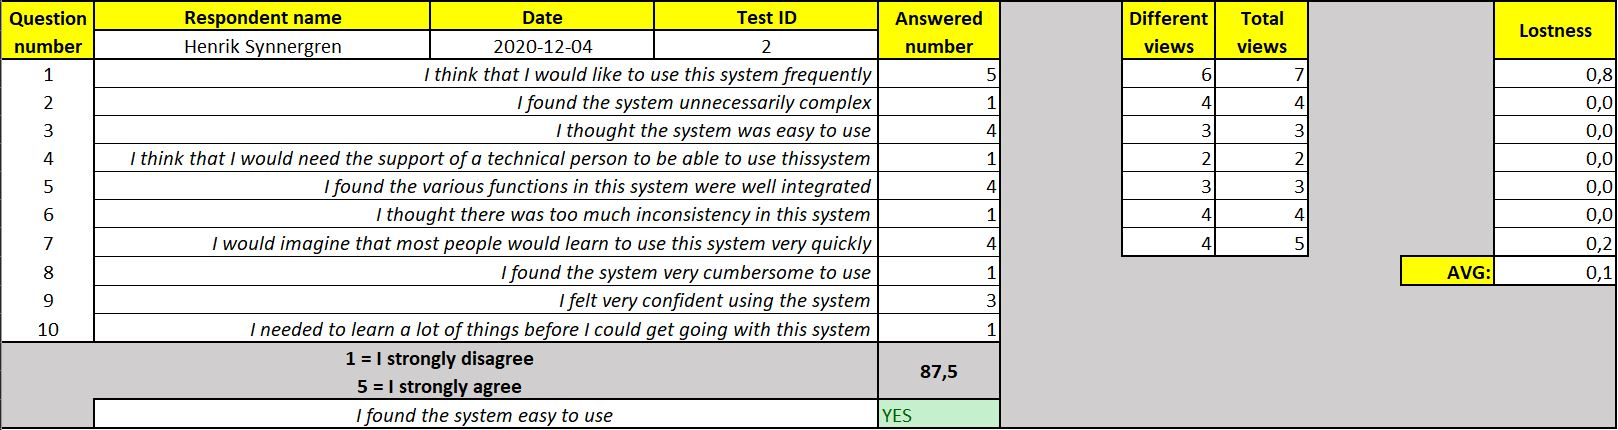
\includegraphics[width=\linewidth]{Pictures/Usertest_2.JPG}
        \caption{Answers from respondent 2}
        \label{fig:Usertest_2}
    \end{figure}
    \begin{figure}[H]
        \centering
        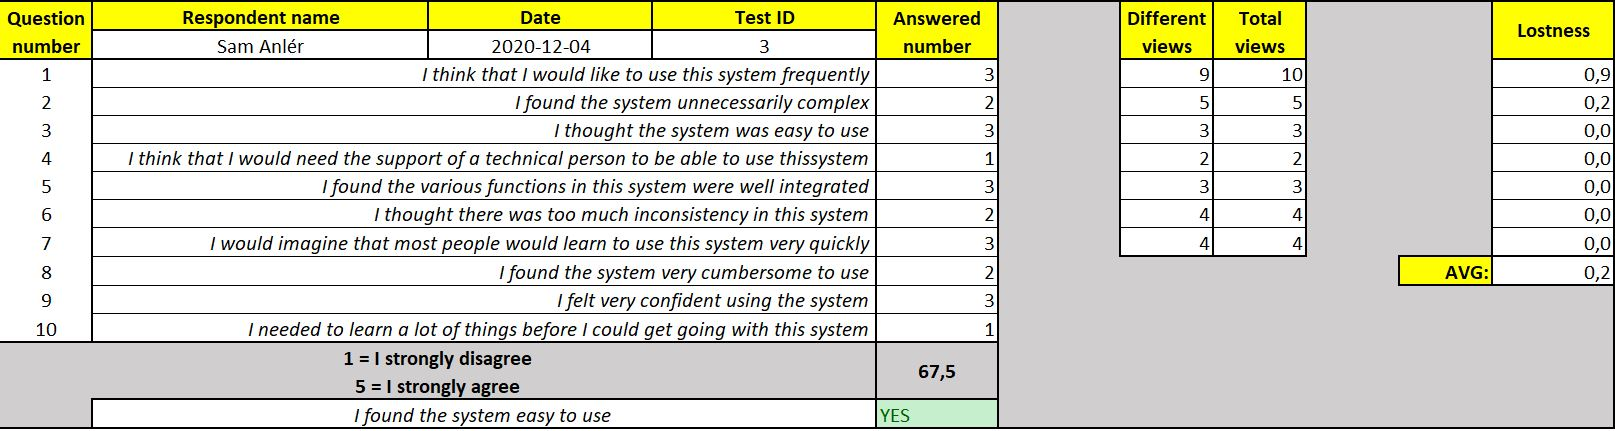
\includegraphics[width=\linewidth]{Pictures/Usertest_3.JPG}
        \caption{Answers from respondent 3}
        \label{fig:Usertest_3}
    \end{figure}
    \begin{figure}[H]
        \centering
        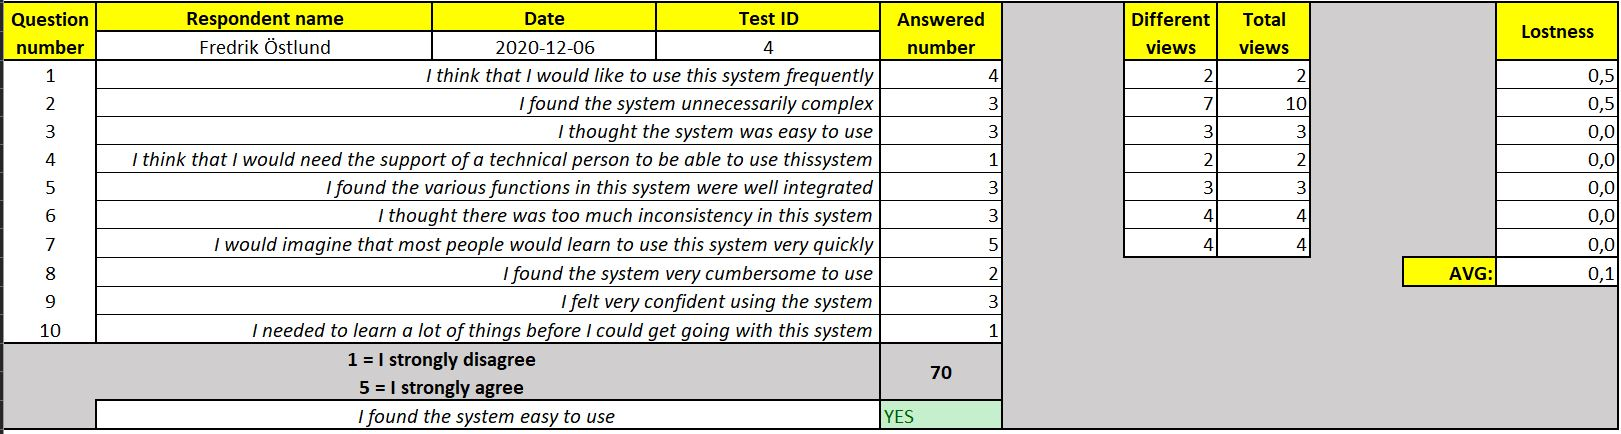
\includegraphics[width=\linewidth]{Pictures/Usertest_4.JPG}
        \caption{Answers from respondent 4}
        \label{fig:Usertest_4}
    \end{figure}
    \begin{figure}[H]
        \centering
        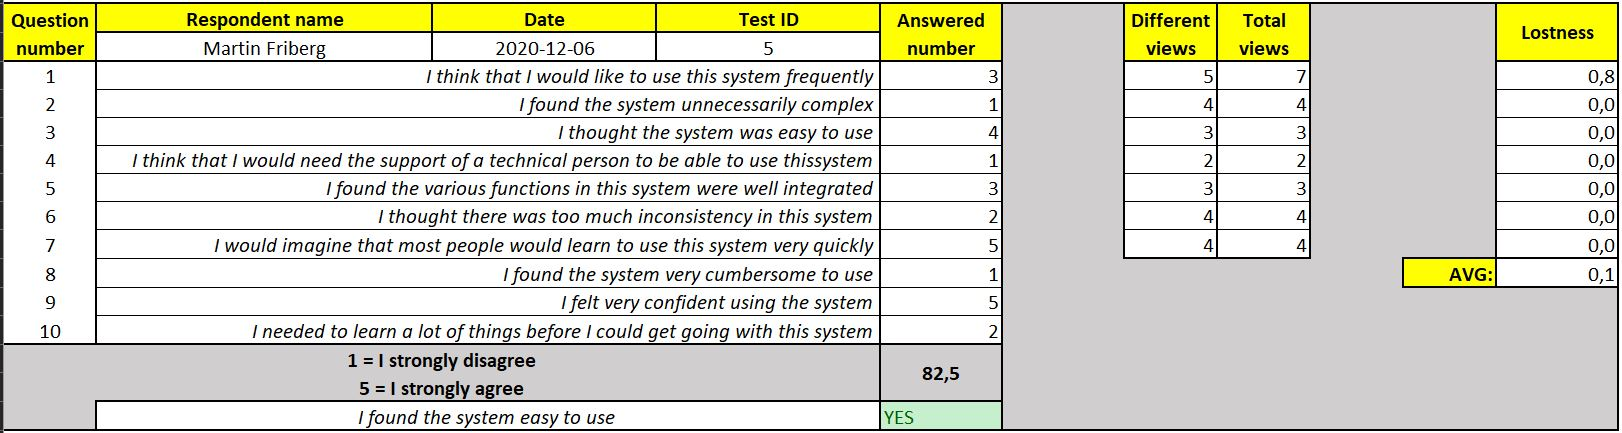
\includegraphics[width=\linewidth]{Pictures/Usertest_5.JPG}
        \caption{Answers from respondent 5}
        \label{fig:Usertest_5}
    \end{figure}
    \begin{figure}[H]
        \centering
        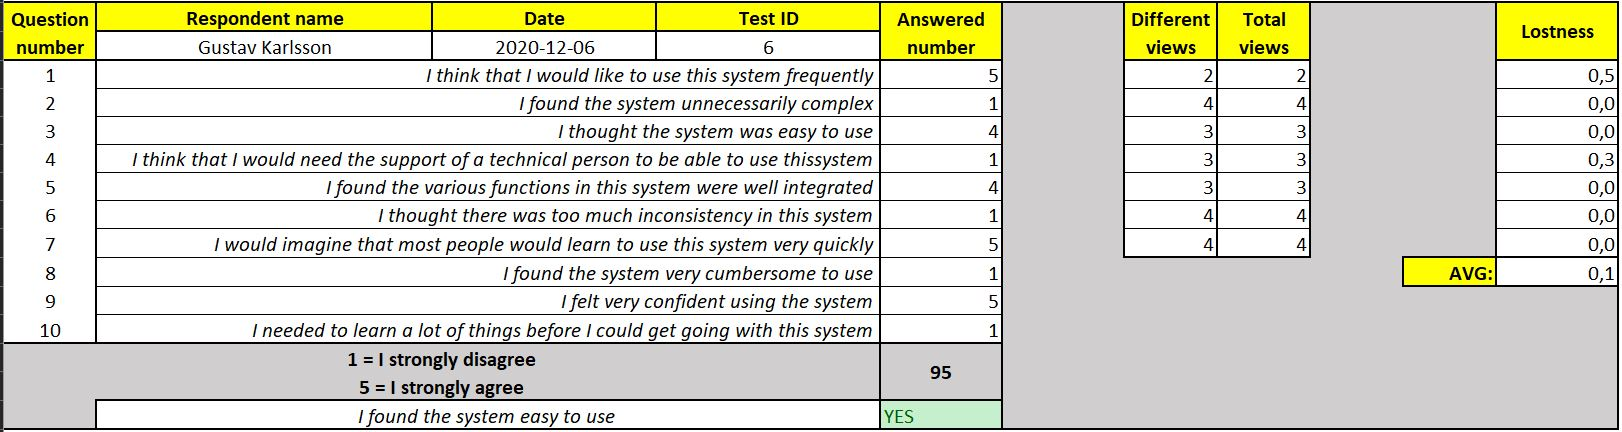
\includegraphics[width=\linewidth]{Pictures/Usertest_6.JPG}
        \caption{Answers from respondent 6}
        \label{fig:Usertest_6}
    \end{figure}
    \begin{figure}[H]
        \centering
        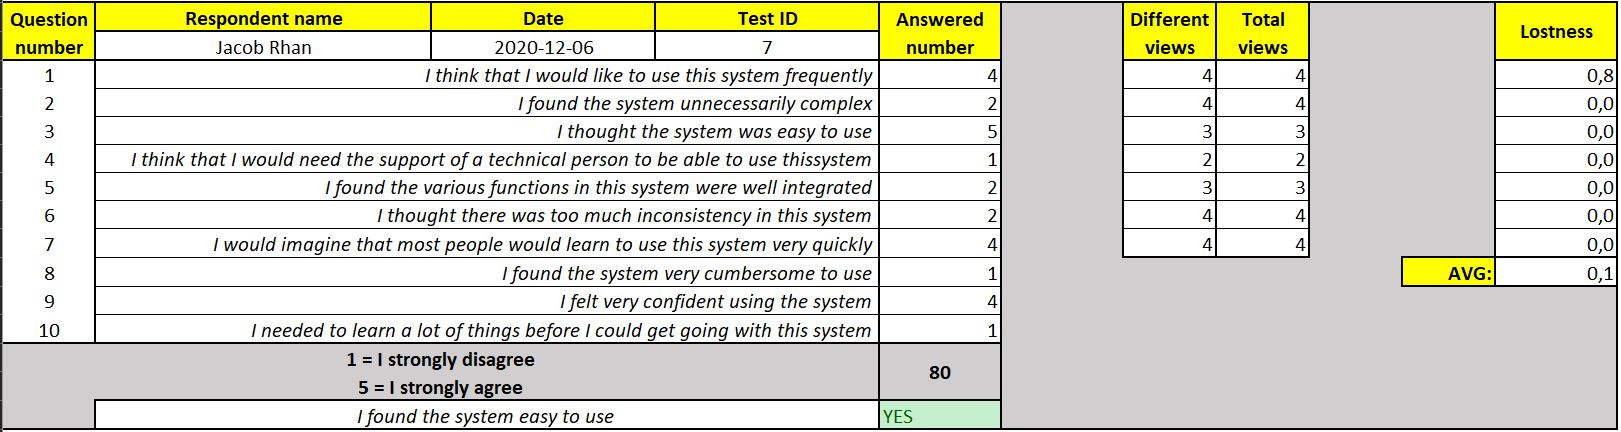
\includegraphics[width=\linewidth]{Pictures/Usertest_7.JPG}
        \caption{Answers from respondent 7}
        \label{fig:Usertest_7}
    \end{figure}
    \begin{figure}[H]
        \centering
        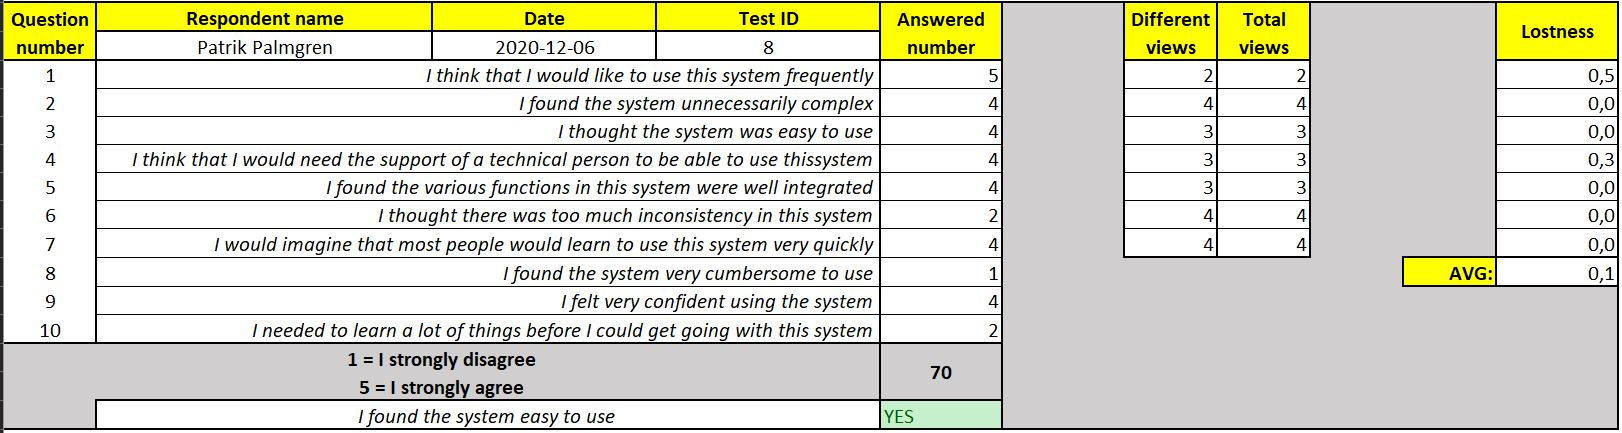
\includegraphics[width=\linewidth]{Pictures/Usertest_8.JPG}
        \caption{Answers from respondent 8}
        \label{fig:Usertest_8}
    \end{figure}
    \begin{figure}[H]
        \centering
        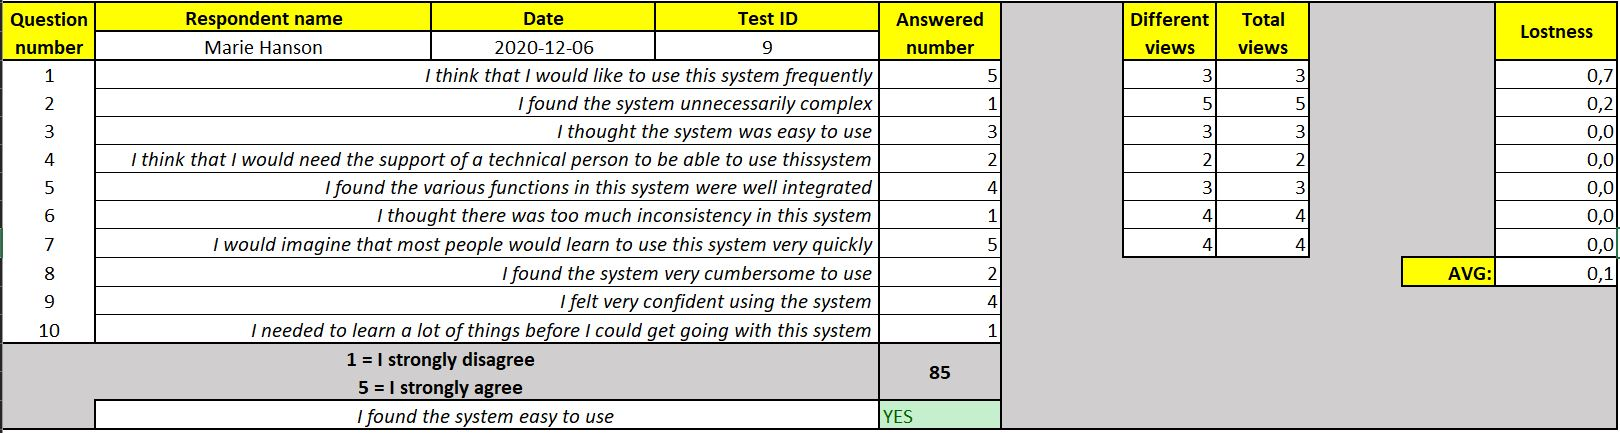
\includegraphics[width=\linewidth]{Pictures/Usertest_9.JPG}
        \caption{Answers from respondent 9}
        \label{fig:Usertest_9}
    \end{figure}
    \begin{figure}[H]
        \centering
        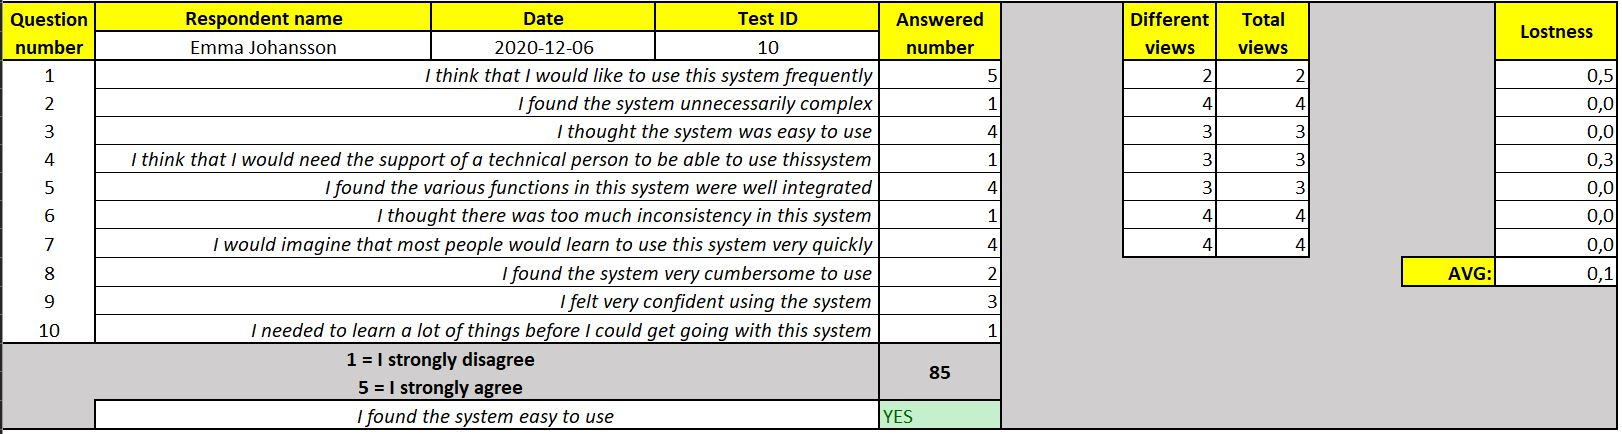
\includegraphics[width=\linewidth]{Pictures/Usertest_10.JPG}
        \caption{Answers from respondent 10}
        \label{fig:Usertest_10}
    \end{figure}
    \subsection{Asked questions in Swedish}
    Below is the list of the statements being used in the test translated to Swedish. 
    \begin{enumerate}
        \item Jag tror att jag skulle vilja använda detta system ofta.
        \item Jag tycker systemet är onödigt komplext.
        \item Jag tycker systemet var lätt att använda.
        \item Jag tror mig behöva hjälp av en tekniskt kunnig och insatt person för att nyttja systemet. 
        \item Jag tycker de olika funktionerna i systemet var väl integrerade.
        \item Jag tycker att det fanns för mycket inkonsekvens i detta system.
        \item Jag skulle tro att de flesta personer skulle lära sig att använda detta system mycket snabbt.
        \item Jag tycker att systemet var mycket besvärligt att använda.
        \item Jag kände mig självsäker när jag använde systemet.
        \item Jag måste lära mig många olika saker innan jag kan använda systemet.
    \end{enumerate}


    
\end{document}